\section{Resultados do desempenho do simulador GPS para a arquitetura baseada 100\% na rede Ethereum}

Para testar o desempenho do simulador GPS para a arquitetura baseada 100\% na rede Ethereum, foi realizado um teste simulando um único GPS que enviava ao contrato a latitude e longitude obtida a cada 1 segundo.

\begin{figure}[h!]
\centering
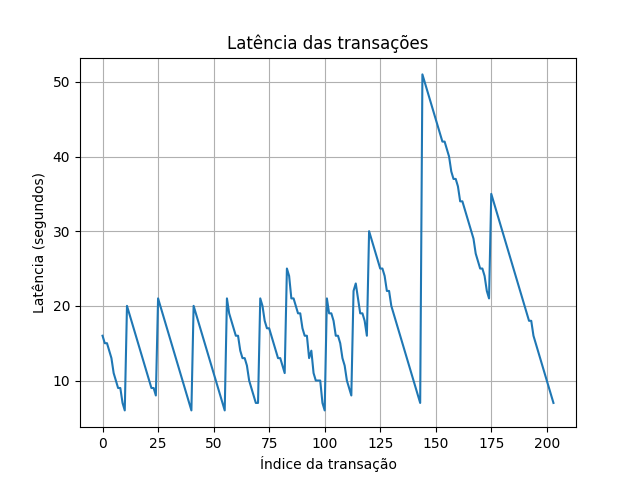
\includegraphics[width=0.7\textwidth]{Cap3/scife_gps_sim_latency.png}
\caption{Latência das transações.}
\label{scife_gps_sim_latency}
\end{figure}

\begin{figure}[h!]
\centering
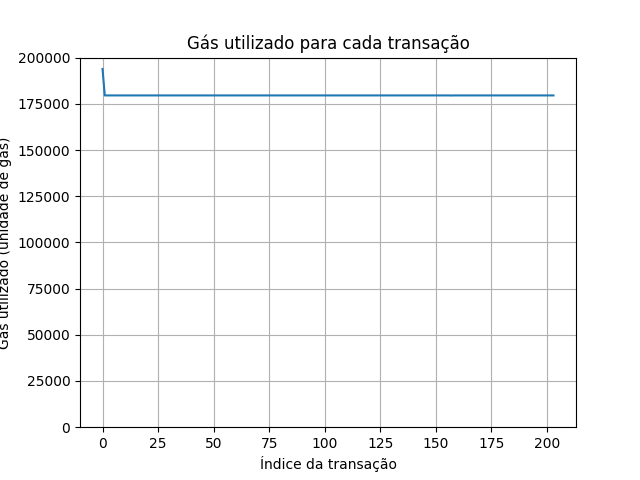
\includegraphics[width=0.7\textwidth]{Cap3/scife_gps_sim_gas_used.png}
\caption{Quantia de gás utilizada por cada transação.}
\label{scife_gps_sim_gas_used}
\end{figure}

\begin{figure}[h!]
\centering
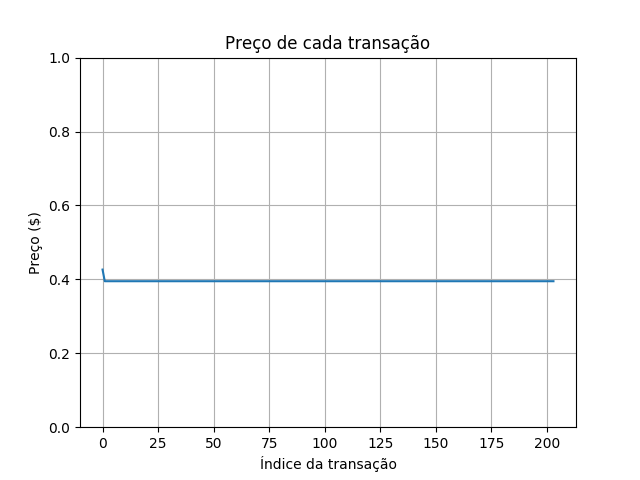
\includegraphics[width=0.7\textwidth]{Cap3/scife_gps_sim_price.png}
\caption{Preço de cada transação}
\label{scife_gps_sim_price}
\end{figure}

Em todos os resultados, para se obter o preço, em dollar, consumido por cada chamada a uma função do contrato, foi considerado que o preço do gás é 10000000000 wei (uma aproximação válida, conforme se vê na figura \ref{gas_price_chart}) e que 1 ETH = \$ 220.00 (uma aproximação válida, conforme se vê na figura \ref{eth_price_chart}).

\begin{figure}[h!]
\centering
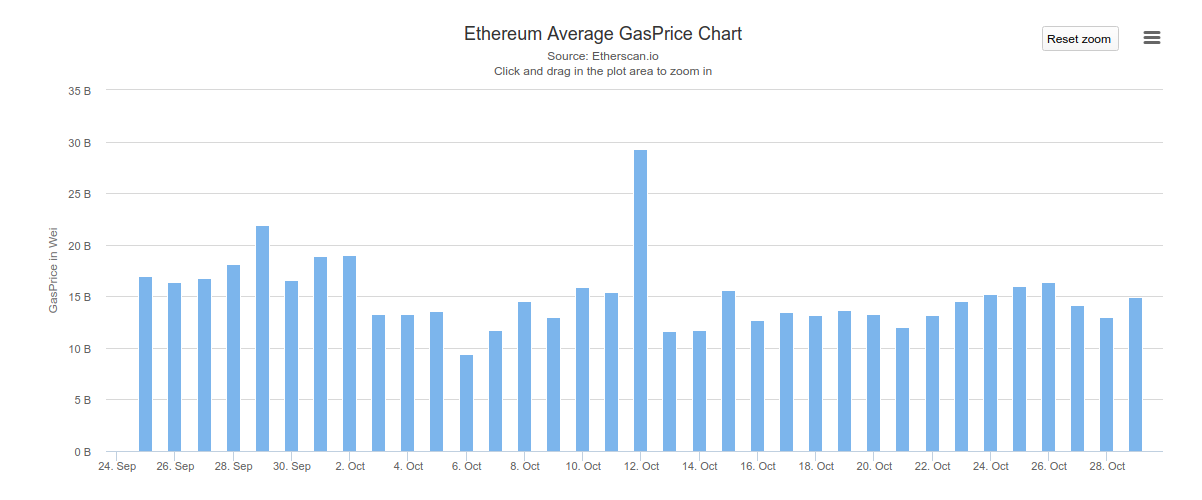
\includegraphics[width=1\textwidth]{Cap3/gas_price_chart}
\caption{Preço dos gás na rede Etherem oficial. Fonte: \href{https://etherscan.io/}{https://etherscan.io/}.}
\label{gas_price_chart}
\end{figure}

\begin{figure}[h!]
\centering
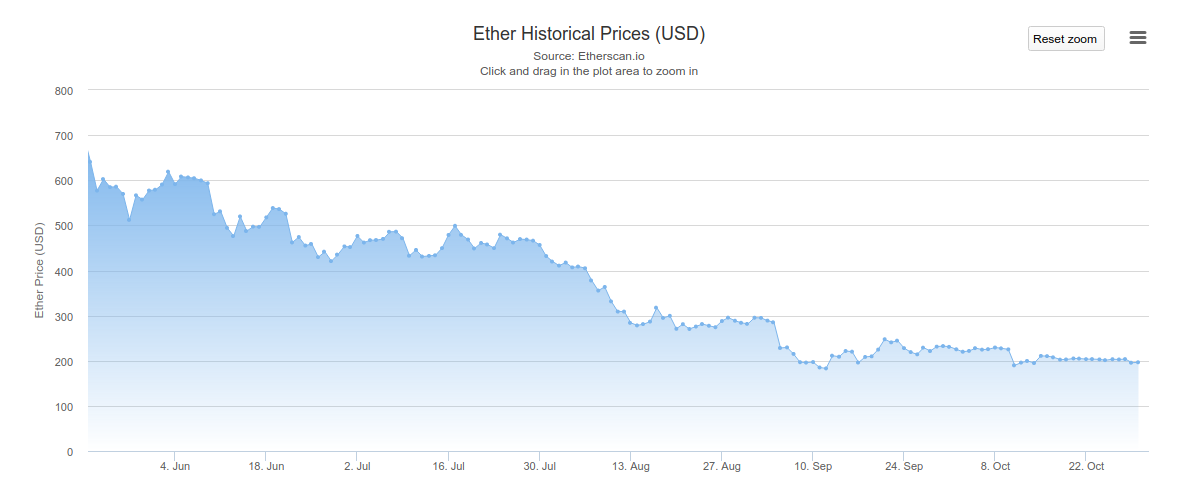
\includegraphics[width=1\textwidth]{Cap3/eth_price_chart}
\caption{Preço do ETH entre Junho e Outubro de 2018. Fonte: \href{https://etherscan.io/}{https://etherscan.io/}.}
\label{eth_price_chart}
\end{figure}

\section{Resultados do desempenho da rede Ethereum para a arquitetura baseada 100\% na rede Ethereum}

Como o contrato está sendo executado nos nós da rede Ethereum, o único valor que nos interessa é a quantia de gás utilizada na chamada de cada uma das funções do contrato. Vale ressaltar que apenas as funções do contrato que modicam os dados internos do contrato consomem gás. As funções que apenas leem os dados internos do contrato (apresentam a palavra chave ``view'' na definição do contrato) não consomem gás. O script que foi utilizado para medir a quantia de gás utilizada por cada função está disponível no GitHub (\href{https://github.com/marcoprado17/scife-calling-all-contract-functions}{https://github.com/marcoprado17/scife-calling-all-contract-functions}).

\begin{table}[h!]
\caption{Quantia de gás consumida por cada uma das funções do contrato.}
\label{my-label}
\begin{center}
\begin{tabular}{cccc}
\hline
Função                   & Parâmetros                                                                         & Gás utilizado & Preço (\$) \\ \hline
enterContract (1º conta) & -                                                                                  & 133043        & 0.2926946  \\ \hline
enterContract (2º conta) & -                                                                                  & 103043        & 0.2266946  \\ \hline
pushGpsData              & \begin{tabular}[c]{@{}c@{}}1540993386,\\ hex string de 64 caracteres\end{tabular}  & 149349        & 0.3285678  \\ \hline
pushGpsData              & \begin{tabular}[c]{@{}c@{}}1540993387,\\ hex string de 64 caracteres\end{tabular}  & 135029        & 0.2970638  \\ \hline
pushGpsData              & \begin{tabular}[c]{@{}c@{}}1540993388,\\ hex string de 128 caracteres\end{tabular} & 179533        & 0.3949726  \\ \hline
pushGpsData              & \begin{tabular}[c]{@{}c@{}}1540993389,\\ hex string de 192 caracteres\end{tabular} & 268541        & 0.5907902  \\ \hline
createNewRefundRequest   & hex string de 64 caracteres                                                        & 164703        & 0.3623466  \\ \hline
createNewRefundRequest   & hex string de 128 caracteres                                                       & 194207        & 0.4272554  \\ \hline
createNewRefundRequest   & hex string de 192 caracteres                                                       & 283215        & 0.623073   \\ \hline
approveRequest           & 0                                                                                  & 66478         & 0.1462516  \\ \hline
confirmBO                & 0                                                                                  & 95190         & 0.209418   \\ \hline
getRefund                & 0                                                                                  & 53696         & 0.1181312  \\ \hline
\end{tabular}
\end{center}
\end{table}

% \begin{center}
% \begin{table}
% \caption{Quantia de gás consumida por cada uma das funções do contrato.}
% \end{table}
% \begin{tabular}{||c c c c||}
% \hline
% Col1 & Col2 & Col2 & Col3 \\ [0.5ex] 
% \hline\hline
% 1 & 6 & 87837 & 787 \\ 
% \hline
% 2 & 7 & 78 & 5415 \\
% \hline
% 3 & 545 & 778 & 7507 \\
% \hline
% 4 & 545 & 18744 & 7560 \\
% \hline
% 5 & 88 & 788 & 6344 \\ [1ex] 
% \hline
% \end{tabular}
% \end{table}
% \end{center}

% \begin{table}[h]
% \centering
% \caption{Quantia de gás consumida por cada uma das funções do contrato.}
% \vspace{0.5cm}
% \begin{tabular}{r|lr}

% Função & Parâmetros & Quantia de gás utilizada & Preço\\ % Note a separação de col. e a quebra de linhas
% \hline                               % para uma linha horizontal
% 1 & Noruega        & .955	& a\\
% 2 & Austrália  	   & .938	& a\\
% 3 & EUA            & .937	& a\\
% 4 & Holanda        & .921	& a\\
% 5 & Alemanha       & .920	& a         % não é preciso quebrar a última linha
 
% \end{tabular}
% \end{table}

\section{Resultados do desempenho do simulador GPS para a arquitetura híbrida}

Para este teste, foi criado um código em NodeJs que simulava o dispositivo GPS. O código está disponível no GitHub (\href{https://github.com/marcoprado17/scih-gps-simulator}{https://github.com/marcoprado17/scih-gps-simulator}). Esse código cria 8 processos e cada processo é responsável por simular 40 dispositivos que ficavam gerando posições de GPS aleatórias e as enviando a cada segundo.





\section{Resultados do desempehnho dos microserviços para arquitetura híbrida}

...
